
%%
%% This is file `sample-sigconf.tex',
%% generated with the docstrip utility.
%%
%% The original source files were:
%%
%% samples.dtx  (with options: `all,proceedings,bibtex,sigconf')
%% 
%% IMPORTANT NOTICE:
%% 
%% For the copyright see the source file.
%% 
%% Any modified versions of this file must be renamed
%% with new filenames distinct from sample-sigconf.tex.
%% 
%% For distribution of the original source see the terms
%% for copying and modification in the file samples.dtx.
%% 
%% This generated file may be distributed as long as the
%% original source files, as listed above, are part of the
%% same distribution. (The sources need not necessarily be
%% in the same archive or directory.)
%%
%%
%% Commands for TeXCount
%TC:macro \cite [option:text,text]
%TC:macro \citep [option:text,text]
%TC:macro \citet [option:text,text]
%TC:envir table 0 1
%TC:envir table* 0 1
%TC:envir tabular [ignore] word
%TC:envir displaymath 0 word
%TC:envir math 0 word
%TC:envir comment 0 0
%%
%% The first command in your LaTeX source must be the \documentclass
%% command.
%%
%% For submission and review of your manuscript please change the
%% command to \documentclass[manuscript, screen, review]{acmart}.
%%
%% When submitting camera ready or to TAPS, please change the command
%% to \documentclass[sigconf]{acmart} or whichever template is required
%% for your publication.
%%
%%
% 
%? \documentclass[sigconf,review,screen]{acmart}
% hyp
\documentclass[sigplan,10pt]{acmart}

\usepackage{listings}     % For ASCII-art / code blocks
\usepackage{booktabs}     % Nicer tables
\usepackage{array}        % Column types
\usepackage{tabularx}     % Automatic column width
\usepackage{enumitem}     % Compact lists



\usepackage{comment}

\usepackage[utf8]{inputenc}
\usepackage[T1]{fontenc}
\usepackage{textcomp}
\usepackage[english]{babel} 
\usepackage{url}
\usepackage{graphicx}


\usepackage{hyperref}       % hyperlinks
\usepackage{amsfonts}       % blackboard math symbols
\usepackage{nicefrac}       % compact symbols for 1/2, etc.
\usepackage{microtype}      % microtypography
\usepackage{xcolor}         % colors
\usepackage{xspace}

%% Define the \sys command for the system name
\newcommand{\sys}{SchedCP\xspace}
%% Define the \agent command for the sched-agent name
\newcommand{\agent}{sched-agent\xspace}

%%
%% \BibTeX command to typeset BibTeX logo in the docs
\AtBeginDocument{%
  \providecommand\BibTeX{{%
    Bib\TeX}}}

\settopmatter{printacmref=false, printccs=false, printfolios=false}
\renewcommand\footnotetextcopyrightpermission[1]{}


%%
%% Submission ID.
%% Use this when submitting an article to a sponsored event. You'll
%% receive a unique submission ID from the organizers
%% of the event, and this ID should be used as the parameter to this command.
%%\acmSubmissionID{123-A56-BU3}

%%
%% For managing citations, it is recommended to use bibliography
%% files in BibTeX format.
%%
%% You can then either use BibTeX with the ACM-Reference-Format style,
%% or BibLaTeX with the acmnumeric or acmauthoryear sytles, that include
%% support for advanced citation of software artefact from the
%% biblatex-software package, also separately available on CTAN.
%%
%% Look at the sample-*-biblatex.tex files for templates showcasing
%% the biblatex styles.
%%

%%
%% The majority of ACM publications use numbered citations and
%% references.  The command \citestyle{authoryear} switches to the
%% "author year" style.
%%
%% If you are preparing content for an event
%% sponsored by ACM SIGGRAPH, you must use the "author year" style of
%% citations and references.
%% Uncommenting
%% the next command will enable that style.
%%\citestyle{acmauthoryear}


%%
%% end of the preamble, start of the body of the document source.
\begin{document}

%%
%% The "title" command has an optional parameter,
%% allowing the author to define a "short title" to be used in page headers.
\title{Towards Agentic OS: An LLM Agent Framework for Linux Schedulers}

\author{Yusheng Zheng}
\email{yzhen165@ucsc.edu}
\affiliation{%
  \institution{University of California, Santa Cruz}
  \city{Santa Cruz}
  \state{California}
  \country{USA}
}

\author{Yanpeng Hu}
\email{huyp@shanghaitech.edu.cn}
\affiliation{%
  \institution{ShanghaiTech University}
  \city{Shanghai}
  \country{China}
}

\author{Wei Zhang}
\email{wei.13.zhang@uconn.edu}
\affiliation{%
  \institution{University of Connecticut}
  \city{Storrs}
  \state{Connecticut}
  \country{USA}
}

\author{Andi Quinn}
\email{aquinn1@ucsc.edu}
\affiliation{%
  \institution{University of California, Santa Cruz}
  \city{Santa Cruz}
  \state{California}
  \country{USA}
}

\begin{abstract}
Operating system schedulers suffer from a fundamental semantic gap, where kernel policies fail to understand application-specific needs, leading to suboptimal performance. We introduce \sys, the first framework that enables fully autonomous Large Language Model (LLM) agents to safely and efficiently optimize Linux schedulers without human involvement. Our core insight is that the challenge is not merely to \emph{apply} a better LLM, but to architect a decoupled control plane that separates the AI's role of semantic reasoning ("what to optimize") from the system's role of execution ("how to observe and act"). Implemented as Model Context Protocol(MCP) server, \sys provides a stable interface with three key services: a Workload Analysis Engine, an evolving Scheduler Policy Repository, and an Execution Verifier that validates all AI-generated code and configure before deployment with static and dynamic analysis. 

We demonstrate this architecture's power with \agent, a multi-agent system that autonomously analyzes workloads, synthesizes custom eBPF scheduling policies, and deploys them via the sched\_ext infrastructure. Our evaluation shows that SchedCP achieves up to an 1.79x performance improvement, and a 13x cost reduction compared to naive agentic approaches, all while maintaining high success rate. By bridging the semantic gap, SchedCP democratizes expert-level system optimization and represents a step towards creating truly self-optimizing, application-aware operating systems. The code is open-sourced in
\href{https://github.com/eunomia-bpf/schedcp}{https://github.com/eunomia-bpf/schedcp}
\end{abstract}


% %%
% %% The code below is generated by the tool at http://dl.acm.org/ccs.cfm.
% %% Please copy and paste the code instead of the example below.
% %%
% \begin{CCSXML}
% <ccs2012>
%  <concept>
%   <concept_id>10010147.10010178.10010187</concept_id>
%   <concept_desc>Computing methodologies~Artificial intelligence</concept_desc>
%   <concept_significance>500</concept_significance>
%  </concept>
%  <concept>
%   <concept_id>10002978.10003006.10003008</concept_id>
%   <concept_desc>Software and its engineering~Operating systems</concept_desc>
%   <concept_significance>300</concept_significance>
%  </concept>
%  <concept>
%   <concept_id>10002978.10003006.10003008.10003010</concept_id>
%   <concept_desc>Software and its engineering~Process scheduling</concept_desc>
%   <concept_significance>500</concept_significance>
%  </concept>
%  <concept>
%   <concept_id>10003033.10003083.10003095</concept_id>
%   <concept_desc>Networks~Cloud computing</concept_desc>

\sloppy


%%
%% This command processes the author and affiliation and title
%% information and builds the first part of the formatted document.
\maketitle

%% Include sections from separate files
\section{Introduction}
\label{sec:intro}

Operating system schedulers face a fundamental challenge: kernel policies cannot understand what applications need. This semantic gap leads to suboptimal performance across modern computing infrastructure. In cloud platforms, system administrators who manage schedulers are not the developers who understand application behavior. On personal devices, regular users lack the expertise to optimize their systems for gaming or creative workloads. Meanwhile, workloads themselves exhibit increasingly dynamic patterns that defy manual optimization.

Prior attempts to automate scheduler optimization, such as those using reinforcement learning~\cite{mao2019decima, qiu2020firm}, have shown promise but remain fundamentally limited. By mapping numerical state to predefined actions, they cannot grasp the semantic intent of a workload and miss optimization opportunities that require deeper reasoning. The advent of Large Language Models (LLMs) Agents, which can automatically reason and use tools for software development, presents an opportunity to bridge this semantic gap, yet a naive approach is impractical. As our motivating experiments reveal, using a powerful agent to generate a basic scheduler from scratch was slow, expensive (\textasciitilde\$6), and resulted in code that often degraded system performance. This highlights a critical gap: existing methods lack semantic understanding, while powerful new models lack the necessary scaffolding for safe, efficient, and reliable systems integration.

To bridge this gap, we introduce a novel, decoupled architecture consisting of two complementary components that leverages AI's unique strengths (semantic reasoning and generative synthesis) while mitigating its weaknesses of cost and unreliability. The first component is \sys, a control plane framework that acts as a safe, stable interface between AI and the kernel \sys\ provides the essential tools for observation, validation, and deployment that any AI agent needs to optimize schedulers. The second component is \agent, our implementation of an autonomous policy engine that leverages a multi-agent LLM system. \agent\ uses the capabilities provided by \sys\ to reason about workloads, synthesize policies, and learn from outcomes.

This architectural separation is fundamental to our approach. \sys\ embodies our core systems contribution: a generalizable framework that can work with any future AI agent, while \agent\ demonstrates the power of this approach through semantic workload analysis and intelligent policy generation. The name `\sys` is inspired by "Context Protocol" (like MCP) and the networking concept of a "Control Plane," reflecting its role as a control plane for AI-driven policy orchestration, separate from the data plane where low-level scheduling decisions execute. Deployed on the production-ready sched\_ext infrastructure, our approach executes with zero LLM overhead in the critical path and makes the following contributions:

\begin{itemize}
    \item \textbf{The \sys\ interface}: A framework that exposes kernel scheduling related features via the Model Context Protocol (MCP), featuring three core services (Workload Analysis Engine, Scheduler Policy Repository, and Execution Verifier) that enable any agent to perform deep semantic analysis of workloads, do AI-driven scheduler optimization without compromising system stability, and learns from experience and improve performance over time.
    \item \textbf{\agent\ multi-agent system}: An autonomous policy engine built on Claude Code's subagent architecture that decomposes scheduler optimization into four specialized agents (Observation, Planning, Execution, and Learning), demonstrating how LLMs can bridge the semantic gap between application requirements and kernel scheduling policies.
    \item \textbf{Evaluation}: We demonstrate that \agent\ achieves up to 1.79× performance improvement on kernel compilation, 50\% latency reduction on scheduler benchmarks, and 88\% cost reduction compared to naive approaches, while maintaining system stability across diverse workloads.
\end{itemize}

Paper organization: Background (§\ref{sec:background}), Motivation (§\ref{sec:motivation}), \sys (§\ref{sec:schedcp_framework}), \agent (§\ref{sec:sched_agents}), Evaluation (§\ref{sec:evaluation}), Related Work (§\ref{sec:related}), Future Work (§\ref{sec:future}), and Conclusion (§\ref{sec:conclusion}).

\section{Background}

\subsection{Evolution of Linux Schedulers}

\subsubsection{Traditional Linux Schedulers}

The Linux kernel has undergone significant evolution in its scheduling subsystem over the past decades. The Completely Fair Scheduler (CFS), introduced in Linux 2.6.23, represents the current default scheduling algorithm and embodies a philosophy of providing "ideal, precise multi-tasking" to all runnable tasks~\cite{wong2008cfs}. CFS models an ideal processor that can run multiple tasks simultaneously, giving each task an equal share of processor time. To approximate this ideal on real hardware, CFS maintains a red-black tree of runnable tasks sorted by their "virtual runtime," ensuring that tasks with the least CPU time are scheduled first.

Beyond CFS, Linux provides real-time scheduling classes including SCHED\_FIFO and SCHED\_RR, which offer deterministic behavior for time-critical applications. These schedulers operate with fixed priorities and preempt normal tasks, making them suitable for embedded systems and real-time applications. However, all these traditional schedulers share a fundamental limitation: they implement one-size-fits-all policies that cannot adapt to specific application requirements or workload characteristics. This inflexibility becomes increasingly problematic as modern computing environments host diverse workloads ranging from latency-sensitive web services to throughput-oriented batch processing jobs.

\subsubsection{sched\_ext (Scheduler Extensions)}

The recent introduction of sched\_ext in Linux 6.12 marks a paradigm shift in kernel scheduler development~\cite{schedext2024}. This framework enables developers to implement custom schedulers as BPF programs that can be dynamically loaded into the kernel without requiring kernel modifications or reboots. The significance of this advancement cannot be overstated: for the first time in Linux history, scheduler development can proceed at user-space velocity while maintaining kernel-level performance and safety.

The sched\_ext framework provides a comprehensive set of callbacks that allow BPF schedulers to control all aspects of task scheduling. These include task enqueueing, CPU selection, load balancing, and idle CPU management. The framework ensures production readiness through minimal overhead—typically less than 1\% in real-world workloads—while providing safety guarantees through BPF verification. This combination of flexibility, safety, and performance makes sched\_ext an ideal platform for experimenting with novel scheduling algorithms, including those generated by AI agents.

\subsubsection{eBPF Technology}

Extended Berkeley Packet Filter (eBPF) has evolved from its origins as a packet filtering mechanism into a general-purpose in-kernel virtual machine that enables safe execution of user-provided programs in kernel space~\cite{mccanne1993bpf,gregg2019bpf}. The eBPF verifier performs extensive static analysis to ensure that programs cannot crash the kernel, access invalid memory, or enter infinite loops. This verification process examines all possible execution paths and enforces strict bounds on loop iterations and memory accesses.

The Just-In-Time (JIT) compilation of eBPF bytecode to native machine instructions ensures near-native performance, making eBPF suitable for performance-critical paths like scheduling. The technology has already transformed multiple kernel subsystems including networking, tracing, and security. Its application to scheduling through sched\_ext represents a natural evolution that brings the same benefits of programmability and safety to the scheduler subsystem. The rich ecosystem of eBPF tools, including bpftool, libbpf, and various tracing utilities, provides a mature foundation for developing and debugging scheduler implementations.

\subsubsection{Infrastructure Challenges}

Modern computing infrastructure faces unprecedented scheduling challenges that traditional approaches cannot adequately address. In cloud environments, the separation between system administrators who configure schedulers and application developers who understand workload requirements creates a fundamental knowledge gap. System administrators must optimize for diverse workloads without deep understanding of application behavior, while developers lack the kernel expertise to influence scheduling decisions.

The heterogeneity of modern workloads further complicates scheduling. A single machine might simultaneously run latency-critical web services requiring microsecond-level response times, batch processing jobs optimizing for throughput, and machine learning workloads alternating between compute-intensive and communication-intensive phases. Static scheduling policies cannot adapt to these dynamic requirements, leading to suboptimal performance and resource utilization. Studies show that many HPC centers achieve less than 50\% utilization due to conservative scheduling policies~\cite{feitelson2023utilization}, while cloud providers report similar inefficiencies in resource allocation.

\subsubsection{Emerging Workload Types}

The computing landscape has evolved dramatically with the rise of new workload paradigms. Machine learning and AI workloads present unique challenges with their alternating phases of compute-intensive training and memory-bound inference. These workloads often exhibit bursty behavior and require careful coordination between CPU and accelerator scheduling. Serverless and Function-as-a-Service platforms introduce extreme dynamism, with functions executing for milliseconds to seconds and requiring rapid cold-start optimization.

Microservices architectures decompose applications into hundreds of interconnected services, each with distinct performance requirements and complex communication patterns. This creates scheduling challenges around tail latency optimization and resource isolation. Batch processing systems have also evolved, now handling jobs ranging from seconds to days with varying resource requirements and deadline constraints. Traditional schedulers struggle to optimize across this diversity, often resulting in conservative resource allocation that leaves significant performance on the table.

\subsubsection{Performance Requirements}

Different application classes impose fundamentally different requirements on the scheduler. Latency-sensitive applications like web services and databases require predictable, low-latency scheduling decisions, often needing response times under 100 microseconds. These workloads benefit from dedicated CPU resources and minimal context switching. In contrast, throughput-oriented workloads such as batch processing and analytics jobs can tolerate higher latencies but require efficient resource utilization and fair sharing across multiple jobs.

Resource-efficient scheduling becomes critical in edge computing and IoT environments where power consumption and thermal constraints dominate. These systems need schedulers that can dynamically adjust performance based on available resources and environmental conditions. Application-specific workloads like build systems and testing suites present unique optimization opportunities—for instance, prioritizing compilation tasks based on dependency graphs can significantly reduce build times. The diversity of these requirements underscores the need for adaptive scheduling approaches that can be tailored to specific workload characteristics.

\subsection{AI/ML in Systems Optimization}

\subsubsection{Reinforcement Learning for OS}

The application of reinforcement learning to operating system optimization has gained significant momentum in recent years, with several high-profile successes demonstrating the potential of learned policies. Decima~\cite{mao2019decima}, presented at SIGCOMM 2019, pioneered the use of graph neural networks for datacenter job scheduling, learning to optimize job completion times by considering complex dependencies between tasks. The system demonstrated improvements of up to 40\% in average job completion time compared to traditional heuristics.

Firm~\cite{qiu2020firm}, published at OSDI 2020, extended RL techniques to multi-resource cluster management with fairness constraints. By modeling the cluster state as a multi-agent system, Firm learns policies that balance resource efficiency with fairness guarantees. More recent work like Park~\cite{mao2019park} provides a platform for applying RL to various computer systems problems, demonstrating the generality of the approach.

However, these RL-based systems face fundamental limitations that motivate our work. First, they require extensive training for each specific workload or environment, often needing millions of scheduling decisions to converge to good policies. Second, they cannot leverage domain knowledge or understand application semantics—they operate purely on statistical patterns in the data. Third, the learned policies are typically black boxes that provide no explanation for their decisions, making debugging and trust difficult. Most critically, they miss optimization opportunities that require semantic understanding, such as recognizing that certain tasks in a compilation pipeline can be prioritized based on dependency analysis.

\subsubsection{LLMs for Code Generation}

The emergence of large language models has revolutionized code synthesis, with systems like Codex~\cite{chen2021codex} (powering GitHub Copilot), GPT-4~\cite{openai2023gpt4}, and Claude~\cite{anthropic2024claude} demonstrating remarkable abilities to generate complex systems code from natural language descriptions. These models have been trained on vast corpora including documentation, code repositories, and technical discussions, giving them deep understanding of programming patterns and system design principles.

Recent evaluations show that LLMs can successfully generate various types of systems code, from device drivers to network protocols. Their ability to understand context and leverage learned patterns makes them particularly suitable for tasks that require domain knowledge, such as implementing scheduling policies for specific workload types. Unlike traditional program synthesis approaches that rely on formal specifications, LLMs can work from informal descriptions and examples, making them more accessible to non-experts.

The key capabilities that make LLMs suitable for scheduler generation include understanding natural language specifications of performance requirements, generating syntactically and semantically correct systems code, reasoning about performance trade-offs and optimization strategies, and learning from examples in documentation and existing code. These capabilities address precisely the limitations of RL-based approaches, suggesting that combining LLMs with RL could yield superior results.

\subsubsection{AI Agents and Autonomous Systems}

The year 2024 marked an inflection point in AI agent capabilities, with the emergence of fully autonomous coding agents that can understand requirements, generate code, test implementations, and iterate based on feedback. Claude Code represents a prime example of this new generation, capable of autonomously developing complex software projects with minimal human intervention. These agents go beyond simple code completion to engage in genuine software engineering tasks including design, implementation, debugging, and optimization.

GitHub Copilot Workspace extends this concept to repository-wide changes, enabling AI agents to understand entire codebases and make coordinated modifications across multiple files. Devin demonstrates end-to-end software engineering capabilities, from understanding requirements through deployment. These systems combine multiple AI capabilities including natural language understanding, code generation, test synthesis, and error correction into cohesive agents that can tackle complex programming tasks.

The evolution from simple code completion to autonomous agents opens unprecedented opportunities for system optimization. Unlike traditional tools that assist human developers, these agents can work continuously to optimize systems, explore design spaces that humans might not consider, and accumulate knowledge across multiple optimization tasks. Their ability to understand both high-level requirements and low-level implementation details makes them ideal candidates for bridging the semantic gap in scheduler optimization that has long plagued traditional approaches.
\section{Motivation}

\subsection{Key Motivations}

\subsubsection{Domain Knowledge Gap in Modern Infrastructure}

Modern computing infrastructure suffers from a fundamental disconnect between those who understand applications and those who manage systems. In cloud platforms, system administrators responsible for optimizing schedulers operate without deep insight into application behavior. A DevOps engineer configuring Kubernetes scheduler policies may have no knowledge of whether a particular workload is latency-sensitive or throughput-oriented, whether it exhibits phase behavior, or how its resource requirements evolve over time. This knowledge gap leads to conservative, suboptimal scheduling decisions that leave performance on the table.

The problem becomes even more acute for edge computing and personal devices, where the gap between user intent and system configuration is vast. Gaming enthusiasts desire optimal performance for their applications but lack the kernel programming knowledge to implement custom schedulers. Creative professionals using video editing software or 3D rendering applications need workload-specific optimizations but cannot modify kernel code. Edge device operators managing IoT deployments require scheduling policies tailored to their specific sensor data processing patterns but lack systems programming expertise. In serverless environments, the abstraction layers completely hide infrastructure details from developers, making it impossible to communicate scheduling requirements to the underlying system.

LLM agents offer a unique opportunity to bridge this gap. These agents can understand workload patterns and requirements from high-level descriptions, translating user intent into concrete scheduling policies. By democratizing access to expert-level optimization, AI agents make it possible for any user—from cloud operators to individual gamers—to achieve performance previously available only to those with deep kernel expertise.

\subsubsection{Technical Complexity of Scheduler Development}

The development of Linux kernel schedulers requires mastery of multiple complex domains that few developers possess. Kernel programming demands understanding of concurrency primitives, lock-free data structures, and the subtle interactions between different kernel subsystems. BPF development adds another layer of complexity with its verification requirements, limited instruction set, and restrictions on memory access patterns. Developers must also understand CPU architectures, cache hierarchies, NUMA topologies, and how scheduling decisions impact performance across these hardware features.

This steep learning curve creates a significant barrier to entry. Even experienced systems programmers often require months to become productive in kernel scheduler development. The consequence is that scheduler innovation proceeds slowly, limited by the small pool of qualified developers. Many optimization opportunities remain unexplored simply because the cost of implementation exceeds available resources. Organizations with unique workload patterns must either accept suboptimal performance or invest heavily in specialized kernel engineering talent.

\subsubsection{Dynamic Workload Adaptation}

Modern workloads exhibit complex phase behavior that changes faster than human operators can respond. Machine learning training workloads exemplify this challenge: they alternate between compute-intensive forward propagation phases, memory-bandwidth-limited weight updates, and communication-heavy gradient synchronization. Each phase benefits from different scheduling strategies—compute phases need CPU affinity and cache optimization, while communication phases benefit from co-scheduling of related tasks. Web applications experience traffic patterns that vary by orders of magnitude throughout the day, requiring different scheduling approaches for peak versus idle periods. Build systems present another challenge with their complex dependency graphs creating varying levels of parallelism as compilation progresses.

Manual scheduler reconfiguration cannot keep pace with these dynamic patterns. By the time a human operator detects a phase change and adjusts scheduling parameters, the workload may have already transitioned to a different phase. This reactive approach leads to persistent suboptimal performance. AI agents, in contrast, can continuously monitor workload behavior and adapt scheduling policies in real-time, potentially even predicting phase transitions based on historical patterns.

\subsection{Motivation Experiments}

To understand the challenges and opportunities of AI-driven scheduler generation, we conducted experiments using state-of-the-art autonomous coding agents. Our goal was to assess both the feasibility and current limitations of using AI to generate kernel schedulers without human intervention.

\subsubsection{Experiment Setup}

We designed our experiment to reflect a realistic scenario where a user without kernel programming expertise attempts to create a custom scheduler. We provided Claude Code, the most advanced autonomous coding agent available, with a simple prompt: "write a scheduler in eBPF." This minimal specification tests the agent's ability to understand the task, navigate the complex technical requirements, and produce working code. The experimental environment consisted of a Linux 6.12 system with sched\_ext enabled, providing the necessary infrastructure for BPF scheduler development. As a baseline for comparison, we measured the time required for an experienced kernel developer to implement the same basic FIFO scheduler.

\subsubsection{Results}

The AI agent successfully synthesized a functional FIFO scheduler without human intervention, demonstrating that autonomous scheduler generation is indeed feasible. However, the path to success revealed significant challenges that must be addressed for practical deployment.

The quantitative metrics paint a sobering picture of current limitations. The generation process required 33 minutes of wall-clock time, during which the agent made 221 separate API calls to the LLM. The agent underwent more than 15 trial-and-error iterations, encountering various compilation errors, BPF verifier rejections, and runtime failures before producing working code. Throughout this process, the agent initiated 8 web browsing sessions to search for eBPF documentation and consulted Linux kernel source code 12 times. The total cost for this single scheduler generation reached approximately \$6 in API fees.

In stark contrast, an experienced kernel developer completed the same task in just 5 minutes at an estimated cost of \$0.50 based on typical developer hourly rates. The developer required only 1-2 iterations, primarily for testing rather than error correction. This 6.6x time difference and 12x cost difference highlight the efficiency gap that must be closed for AI-driven scheduler generation to become practical.

\subsubsection{Key Observations}

Our analysis of the AI-generated scheduler revealed three critical categories of challenges that must be addressed by any practical framework.

First, code quality issues plague naive AI generation. The AI-generated scheduler exhibited higher overhead than necessary due to inefficient data structure choices, using linked lists where arrays would suffice and performing unnecessary memory allocations in the scheduling hot path. The code showed suboptimal CPU cache usage patterns, with data structures laid out in ways that increase cache misses. Most concerning, the AI missed several optimizations that would be obvious to human experts, such as avoiding lock contention through per-CPU data structures and minimizing scheduler decision complexity. These quality issues meant that despite being functionally correct, the AI-generated scheduler sometimes performed worse than the default CFS scheduler it was meant to improve.

Second, the cost and time requirements make the current approach prohibitive for production use. At \$6 per scheduler generation, organizations would face significant costs for workload-specific optimization. The 33-minute generation time is too slow for dynamic adaptation to changing workloads. The multiple iterations waste computational resources on both the client and server side, contributing to both cost and environmental concerns. These efficiency issues must be addressed through better frameworks and interfaces that guide the AI toward successful implementations more directly.

Third, safety and reliability concerns arise from the autonomous agent's broad system access requirements. The agent required root access to load kernel modules, creating security risks if the agent were compromised. During testing, the agent's generated code could potentially crash the system, requiring manual intervention to recover. The lack of built-in safety checks meant that performance regressions could go unnoticed until production deployment. The absence of gradual rollout mechanisms meant that failures affected the entire system rather than a controlled subset.

\subsection{Research Challenges}

Based on our experimental findings, we identify four critical research challenges that must be addressed to realize the vision of AI-driven scheduler optimization.

\subsubsection{Safety and Reliability}

Ensuring the safety of AI-generated kernel code represents perhaps the most critical challenge. We must guarantee that generated schedulers cannot crash the kernel through null pointer dereferences, infinite loops, or invalid memory accesses. The system must prevent soft-lockups where the scheduler consumes excessive CPU time, priority inversions where low-priority tasks block high-priority ones indefinitely, and starvation where some tasks never receive CPU time. Beyond preventing catastrophic failures, we must minimize negative impacts on production workloads, ensuring that even suboptimal scheduling decisions degrade performance gracefully rather than catastrophically. Finally, the system must provide robust rollback mechanisms that can quickly revert to known-good schedulers when problems are detected.

\subsubsection{Efficiency and Cost}

The current 33-minute generation time must be reduced to seconds for the approach to be practical in dynamic environments. This requires fundamental improvements in how AI agents approach scheduler generation, moving from trial-and-error to more directed synthesis. LLM API costs must be minimized while maintaining generation quality, requiring clever context management and caching strategies. The system must leverage experience from previous scheduler generation to avoid repeating work, building a knowledge base that grows over time. Costs must be amortized across multiple deployments, making workload-specific optimization economically viable for a broader range of users.

\subsubsection{Performance Optimization}

AI-generated code must match or exceed human expert performance to justify deployment. This requires ensuring that the AI understands performance implications of different implementation choices, from data structure selection to algorithm design. The system must automatically incorporate domain-specific optimizations that human experts would apply, such as cache-aware data layouts and lock-free algorithms where appropriate. Performance validation must occur before production deployment, with comprehensive benchmarking that captures both average-case and worst-case behavior. The system must support continuous improvement based on runtime feedback, learning from production performance to generate better schedulers over time.

\subsubsection{Generalization and Adaptability}

The framework must handle diverse workload types without requiring retraining or manual configuration for each new scenario. This demands architectures that can transfer knowledge between similar scheduling problems, recognizing patterns that apply across different but related workloads. As new hardware architectures emerge with different performance characteristics, the system must adapt automatically without requiring framework updates. User-specific requirements and constraints must be incorporated naturally, allowing customization without sacrificing the benefits of automated generation. The system must balance specialization for specific workloads with generalization across workload classes.

These challenges motivate our design principles and system architecture, which we present in the following section. By addressing each challenge systematically, we create a framework that makes AI-driven scheduler optimization both practical and beneficial.
\input{sections/design\_impl}
\section{Evaluation}
\label{sec:evaluation}

% \subsection{Research Questions}

We investigate key research questions to validate the effectiveness and efficiency of \sys:

\begin{itemize}
\item \textbf{RQ1}: Can \sys effectively configure existing schedulers?
\item \textbf{RQ2}: Can \sys generate new schedulers for specific workloads?
\item \textbf{RQ3}: What is the cost and efficiency of \sys's scheduler generation?
\item \textbf{RQ4}: How much can \agent continue to improve performance after initial attempt?
% \item \textbf{RQ5}: How effectively can \sys understand workloads?
\end{itemize}

\subsection{Experimental Setup}

We evaluate \sys on two machines, machine 1 is an 86-core, 172 threads Intel Xeon 6787P with 758GB RAM, NVMe SSDs, 10Gbps network, with 2x 256 GB CXL (Compute Express Link) memory device, 3 numa node, running Linux 6.14 with sched\_ext. Machine 2 is an 8-core, 8 threads Intel Core Ultra 7 258V with 30GB RAM, NVMe SSDs, 1 NUMA node, running Linux 6.13 with sched\_ext. We test Claude Code (Opus 4) as AI agents to validate framework generality. For each case, we test 3 times and get the average results. To mitigate cache warming effects, we clear the page cache (via \texttt{sync; echo 3 > /proc/sys/vm/drop\_caches}) before each run and perform a warm-up run that is excluded from measurements. In all the experiments, the Agent successfully creates working custom scheduler configurations or generates new eBPF programs.

\subsection{AI configured schedulers for kernel build and schbench}

% For schbench, the LLM achieves 50\% lower p99 latency and 30\% higher throughput by selecting scx\_layered. 

We evaluate the \sys and \agent's ability to both select/configure existing schedulers and generate new ones, as well as learn after the first attempt. The iterative refinement simulates realistic deployment scenarios where schedulers are evaluated over multiple runs before production deployment. Note that the attempt counts measure the iteration of the observe-optimization process in the AI Agents, it does not require the workload to be re-run. The Linux kernel build benchmark compiles the kernel 6.14 with tinyconfig and ``make -j 172'' on machine 1. Figure~\ref{fig:performance-comparison} shows performance improvements across three stages: baseline EEVDF, initial AI-selected schedulers, and iteratively-refined configurations. We also compare with pre-trained RL algorithms that have been proposed for scheduler optimization~\cite{corbet2025ml} out of the box, which only tunes scheduler parameter. The workload shows 1.63x speedup from 13.57s to 8.31s using scx\_rusty as the first attempt. After 3 iterations of observe-optimization process, the \agent selects the scx\_layered scheduler and adds 16\% additional gain beyond LLM configuration, with total improvements of 1.79x over baseline EEVDF. In contrast, basic RL approaches show no improvement in our tests, likely because they require hardware or workload-specific retraining, which is costly and time-consuming.

\begin{figure}[h]
\centering
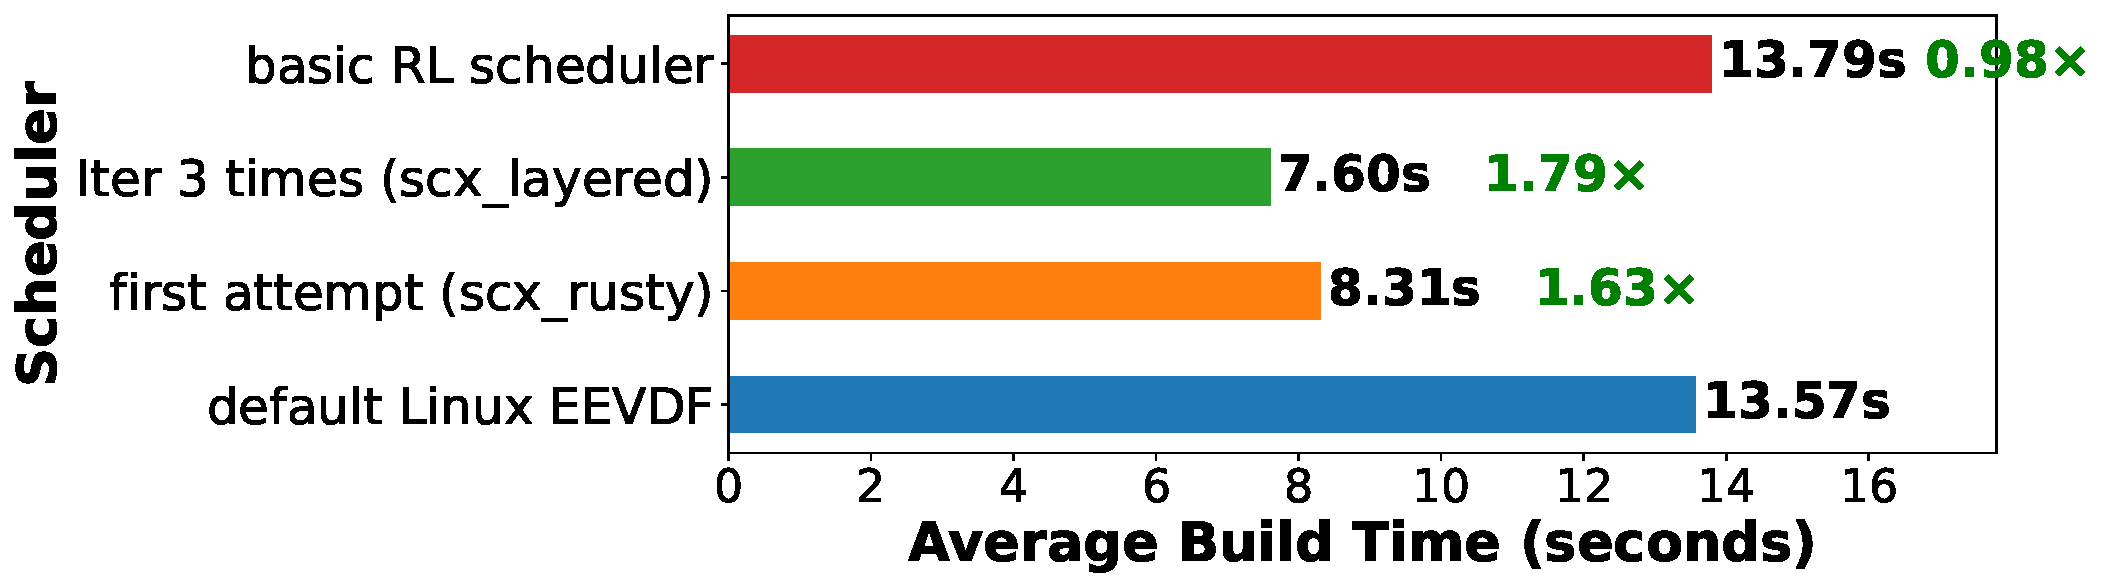
\includegraphics[width=0.9\columnwidth]{sections/Linux_build_benchmark_results.pdf}
\caption{Performance comparison of scheduler configurations in Linux build benchmark.}
\label{fig:performance-comparison}
\end{figure}

We further evaluate \sys on machine 2 using schbench~\cite{schbench2016}, a scheduler benchmark measuring wakeup latency and throughput. Figure~\ref{fig:schbench-comparison} compares three configurations: default EEVDF, initial selection (scx\_bpfland), and iterative optimization (scx\_rusty after 3 iterations). While AI configured scheduler initially underperformed with 13\% worse P99 latency (46.1ms vs 40.3ms) and 19\% lower throughput (741 vs 910 req/s), AI iterative refinement identified scx\_rusty as superior. After three iterations, scx\_rusty achieved 2.11× better P99 latency (19.1ms) and 1.60× higher throughput (1452 req/s) versus EEVDF, demonstrating our agent's effective learning from performance feedback.

\begin{figure}[h]
\centering
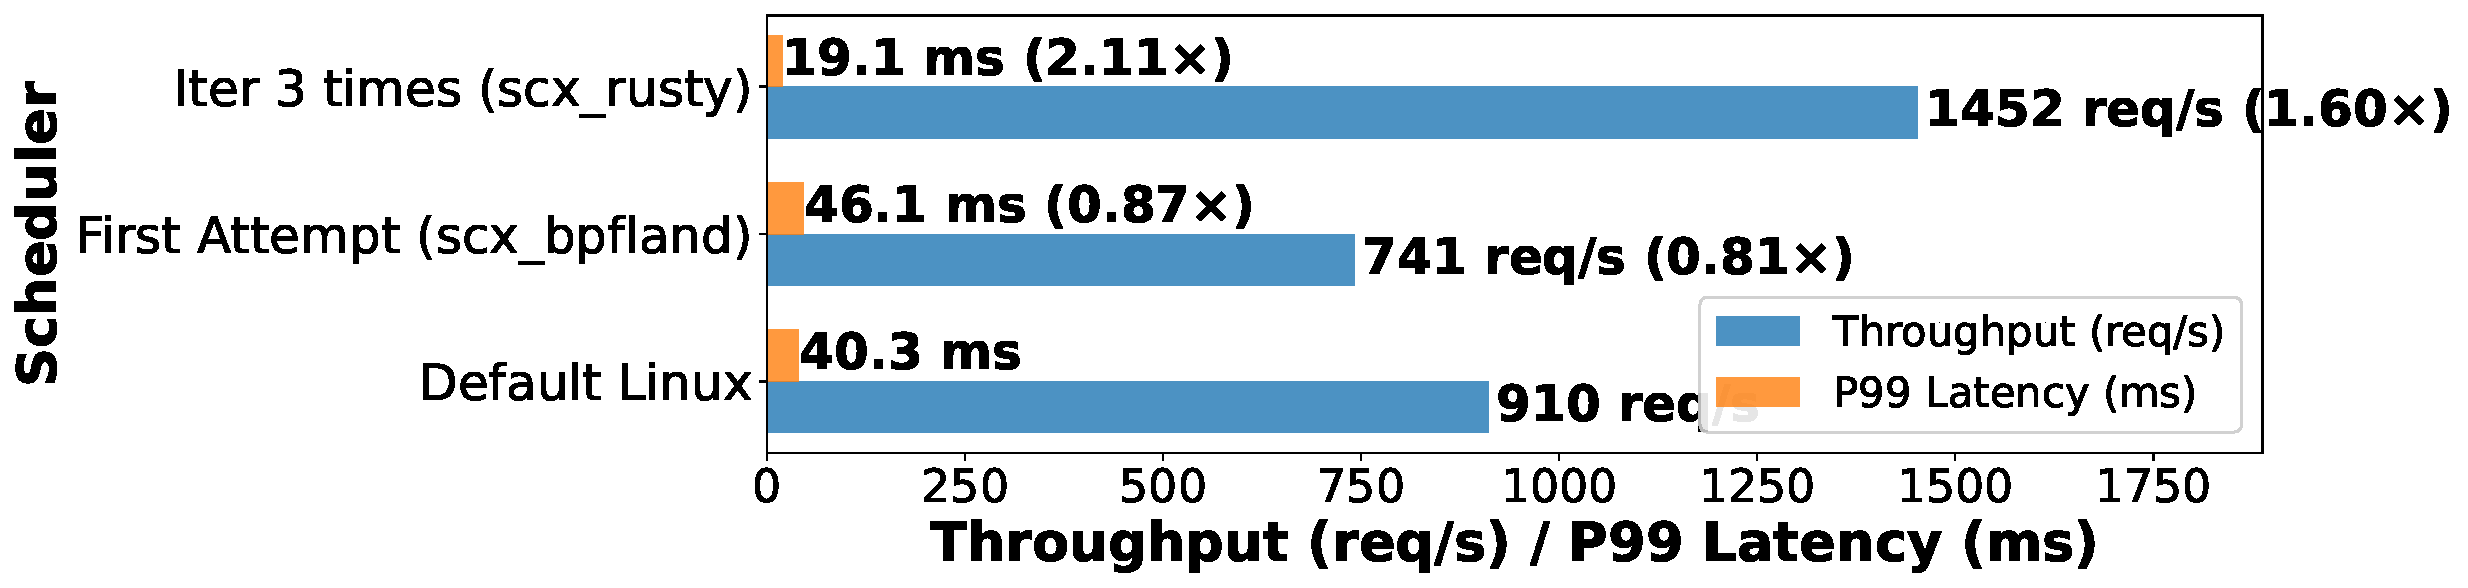
\includegraphics[width=0.9\columnwidth]{sections/schbench_performance_comparison.pdf}
\caption{Schbench performance comparison showing P99 latency and throughput improvements through iterative scheduler optimization.}
\label{fig:schbench-comparison}
\end{figure}

\subsection{AI-Generated Schedulers for Batch Workloads}

Figure~\ref{fig:batch-performance} evaluates the \sys  and \agent  ability to generate new schedulers from scratch (not merely select existing ones) on 8 diverse batch workloads (e.g. file compression, video transcoding, software testing, and data analytics tasks) running on machine 2. To simulate a long-tail distribution, each workload comprised 40 parallel tasks: 39 short and one significantly longer, each as a python script or C/C++ program. The agent consistently identified this pattern and generated custom eBPF code implementing a Longest Job First (LJF) scheduling policy—a scheduler not present in our repository—achieving an average 20\% reduction in end-to-end processing time. The cost for this analysis averaged \$0.15 per workload, based on Claude Opus 4 pricing from August 2025. We note that the powerful Claude Opus agent successfully classified all 8 workloads, whereas the smaller Claude Sonnet model could not. In addition to performance gains, our framework's optimizations reduced generation costs per iteration: time fell from 33 to 2.5 minutes (a 13x reduction), and the monetary cost dropped from \$6 to \$0.5.

\begin{figure}[h]
\centering
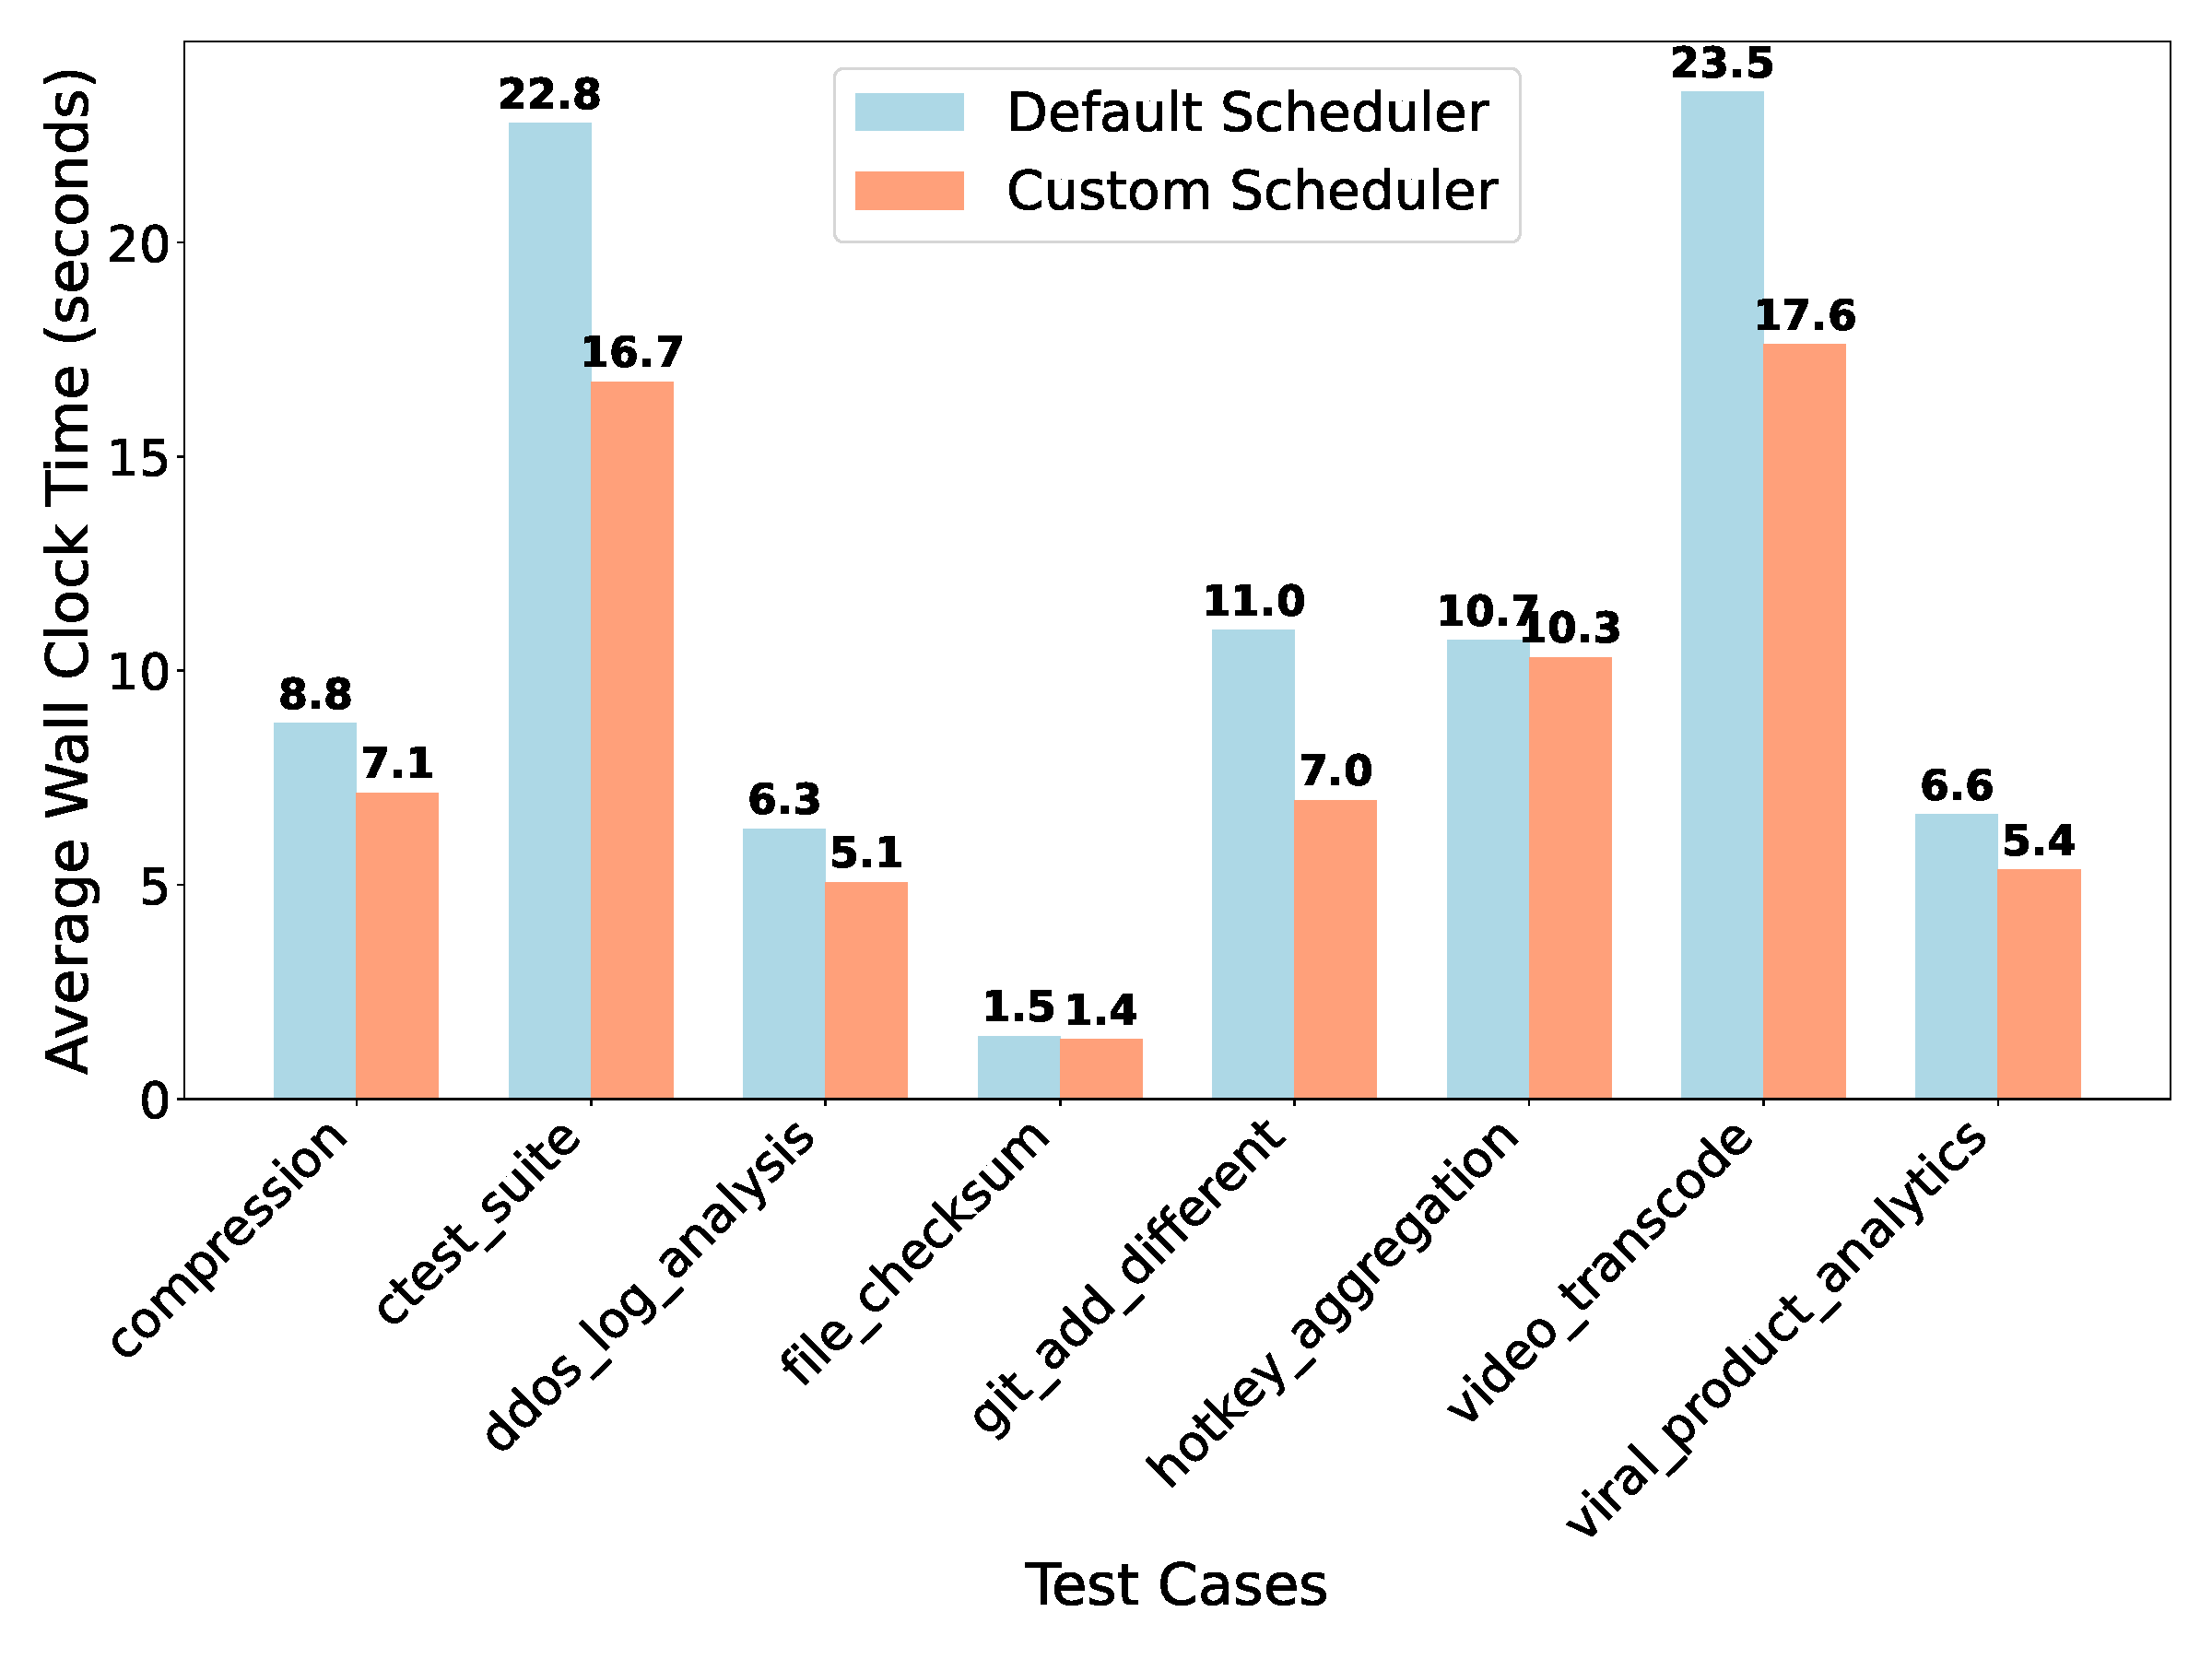
\includegraphics[width=0.9\columnwidth]{sections/scheduler_performance_comparison.pdf}
\caption{AI-generated scheduler performance on batch workloads.}
\label{fig:batch-performance}
\end{figure}



\section{Related Work}
\label{sec:related}

Machine learning has a history of optimizing systems, including learned indexes~\cite{kraska2018learned}, database tuning~\cite{marcus2019neo,vanaken2017ottertune}, and RL-based job schedulers~\cite{mao2019decima,qiu2020firm,zhang2024mrsch} supported by platforms like Park~\cite{mao2019park}. However, these methods require extensive training, lack the semantic understanding to transfer knowledge across diverse workloads, or need human specify high level optimization goals. While recent work has applied LLMs to system diagnostics~\cite{wang2024llmsys} and  code generation~\cite{wei2024mapper,10.1145/3672197.3673434}, our work is the first to use an autonomous agent to design, configure and generate kernel schedulers, and apply them for end-to-end system optimization without human involvement. By leveraging LLM Agent reasoning, tool usage with sched\_ext and eBPF, our framework uniquely bridges the semantic gap between application needs and system policy.

% Machine learning has transformed fundamental system components. Learned indexes~\cite{kraska2018learned} replace B-trees with neural networks, achieving up to 70\% memory savings and 3x lookup performance improvements. In scheduling specifically, Decima~\cite{mao2019decima} uses graph neural networks for datacenter job scheduling, reducing completion time by 40\%, while Firm~\cite{qiu2020firm} addresses multi-resource cluster scheduling with fairness constraints, improving utilization by 25-30\%. MrSch~\cite{zhang2024mrsch} extends these approaches achieving up to 48\% performance improvements. Park~\cite{mao2019park} provides a general platform for applying RL to systems problems. Beyond scheduling, Neo~\cite{marcus2019neo} applies deep RL to database query optimization, achieving 2x performance improvements, while OtterTune~\cite{vanaken2017ottertune} uses Gaussian Process regression to tune database configurations, reaching 94\% of expert DBA performance. However, these approaches share fundamental limitations: they require extensive training (millions of decisions), cannot transfer knowledge between workloads, and operate on statistical patterns without semantic understanding. Recent work demonstrates LLMs' potential in systems optimization. Wang et al.~\cite{wang2024llmsys} show GPT-4 diagnosing 78\% of distributed system problems, and mapper generation~\cite{wei2024mapper} achieves 3.8× speedups for parallel programs, though in constrained domains. Our work uniquely combines semantic understanding with production readiness: unlike RL approaches learning from scratch or auto-tuners optimizing parameters, we leverage LLMs' pre-trained knowledge to generate entirely new scheduling algorithms through an autonomous optimization loop. Built on sched\_ext with eBPF safety guarantees, our self-evolving scheduler library accumulates knowledge across workloads, representing the first AI agents generating production-quality kernel schedulers from natural language requirements.
\section{Future Work}
\label{sec:future}

While \sys demonstrates the viability of AI-driven scheduler optimization, extending our framework beyond schedulers to cache policies, DVFS, network configuration, and sysctl parameters presents immediate opportunities for a unified OS optimization framework. Cross-component optimization, where CPU, memory, I/O, and power decisions inform each other, could unlock significant performance gains through new abstractions for expressing inter-component dependencies. The broader impact extends beyond technical improvements: \sys democratizes OS optimization by enabling application-specific kernel policies without requiring kernel expertise, effectively bridging the gap between application needs and kernel capabilities. This work opens new possibilities for adaptive, application-aware operating systems that can automatically optimize themselves for changing workloads, making expert-level performance accessible to all users.
\section{Conclusion}
\label{sec:conclusion}

In this paper, we introduced \sys, the first framework designed to empower autonomous LLM agents to safely and efficiently optimize Linux schedulers. Our core contribution is a decoupled control plane architecture that cleanly separates the AI's role of semantic reasoning from the system's role of safe execution, bridging the critical semantic gap between application needs and kernel policy. We demonstrated through \agent that this approach not only achieves significant performance improvements up to a 1.79× speedup and an 88\% cost reduction over naive agentic methods, but also maintains system stability by autonomously synthesizing and deploying custom eBPF scheduling policies. By providing a stable, verifiable interface for AI-driven optimization, SchedCP represents a foundational step towards a new generation of agentic, self-optimizing operating systems that are truly application-aware.









%%
%% The acknowledgments section is defined using the "acks" environment
%% (and NOT an unnumbered section). This ensures the proper
%% identification of the section in the article metadata, and the
%% consistent spelling of the heading.
% \begin{acks}
% This work was supported in part by...
% \end{acks}

%%
%% The next two lines define the bibliography style to be used, and
%% the bibliography file.
\bibliographystyle{ACM-Reference-Format}
\bibliography{sample-base}

\end{document}

This document will explain the major features of the document
class. For further information, the {\itshape \LaTeX\ User's Guide} is
available from
\url{https://www.acm.org/publications/proceedings-template}.

\subsection{Template Styles}

The primary parameter given to the ``\verb|acmart|'' document class is
the {\itshape template style} which corresponds to the kind of publication
or SIG publishing the work. This parameter is enclosed in square
brackets and is a part of the {\verb|documentclass|} command:
\begin{verbatim}
  \documentclass[STYLE]{acmart}
\end{verbatim}

Journals use one of three template styles. All but three ACM journals
use the {\verb|acmsmall|} template style:
\begin{itemize}
\item {\texttt{acmsmall}}: The default journal template style.
\item {\texttt{acmlarge}}: Used by JOCCH and TAP.
\item {\texttt{acmtog}}: Used by TOG.
\end{itemize}

The majority of conference proceedings documentation will use the {\verb|acmconf|} template style.
\begin{itemize}
\item {\texttt{sigconf}}: The default proceedings template style.
\item{\texttt{sigchi}}: Used for SIGCHI conference articles.
\item{\texttt{sigplan}}: Used for SIGPLAN conference articles.
\end{itemize}

\subsection{Template Parameters}

In addition to specifying the {\itshape template style} to be used in
formatting your work, there are a number of {\itshape template parameters}
which modify some part of the applied template style. A complete list
of these parameters can be found in the {\itshape \LaTeX\ User's Guide.}

Frequently-used parameters, or combinations of parameters, include:
\begin{itemize}
\item {\texttt{anonymous,review}}: Suitable for a ``double-anonymous''
  conference submission. Anonymizes the work and includes line
  numbers. Use with the \texttt{\string\acmSubmissionID} command to print the
  submission's unique ID on each page of the work.
\item{\texttt{authorversion}}: Produces a version of the work suitable
  for posting by the author.
\item{\texttt{screen}}: Produces colored hyperlinks.
\end{itemize}

This document uses the following string as the first command in the
source file:
\begin{verbatim}
\documentclass[sigconf]{acmart}
\end{verbatim}

\section{Modifications}

Modifying the template --- including but not limited to: adjusting
margins, typeface sizes, line spacing, paragraph and list definitions,
and the use of the \verb|\vspace| command to manually adjust the
vertical spacing between elements of your work --- is not allowed.

{\bfseries Your document will be returned to you for revision if
  modifications are discovered.}

\section{Typefaces}

The ``\verb|acmart|'' document class requires the use of the
``Libertine'' typeface family. Your \TeX\ installation should include
this set of packages. Please do not substitute other typefaces. The
``\verb|lmodern|'' and ``\verb|ltimes|'' packages should not be used,
as they will override the built-in typeface families.

\section{Title Information}

The title of your work should use capital letters appropriately -
\url{https://capitalizemytitle.com/} has useful rules for
capitalization. Use the {\verb|title|} command to define the title of
your work. If your work has a subtitle, define it with the
{\verb|subtitle|} command.  Do not insert line breaks in your title.

If your title is lengthy, you must define a short version to be used
in the page headers, to prevent overlapping text. The \verb|title|
command has a ``short title'' parameter:
\begin{verbatim}
  \title[short title]{full title}
\end{verbatim}

\section{Authors and Affiliations}

Each author must be defined separately for accurate metadata
identification.  As an exception, multiple authors may share one
affiliation. Authors' names should not be abbreviated; use full first
names wherever possible. Include authors' e-mail addresses whenever
possible.

Grouping authors' names or e-mail addresses, or providing an ``e-mail
alias,'' as shown below, is not acceptable:
\begin{verbatim}
  \author{Brooke Aster, David Mehldau}
  \email{dave,judy,steve@university.edu}
  \email{firstname.lastname@phillips.org}
\end{verbatim}

The \verb|authornote| and \verb|authornotemark| commands allow a note
to apply to multiple authors --- for example, if the first two authors
of an article contributed equally to the work.

If your author list is lengthy, you must define a shortened version of
the list of authors to be used in the page headers, to prevent
overlapping text. The following command should be placed just after
the last \verb|\author{}| definition:
\begin{verbatim}
  \renewcommand{\shortauthors}{McCartney, et al.}
\end{verbatim}
Omitting this command will force the use of a concatenated list of all
of the authors' names, which may result in overlapping text in the
page headers.

The article template's documentation, available at
\url{https://www.acm.org/publications/proceedings-template}, has a
complete explanation of these commands and tips for their effective
use.

Note that authors' addresses are mandatory for journal articles.

\section{Rights Information}

Authors of any work published by ACM will need to complete a rights
form. Depending on the kind of work, and the rights management choice
made by the author, this may be copyright transfer, permission,
license, or an OA (open access) agreement.

Regardless of the rights management choice, the author will receive a
copy of the completed rights form once it has been submitted. This
form contains \LaTeX\ commands that must be copied into the source
document. When the document source is compiled, these commands and
their parameters add formatted text to several areas of the final
document:
\begin{itemize}
\item the ``ACM Reference Format'' text on the first page.
\item the ``rights management'' text on the first page.
\item the conference information in the page header(s).
\end{itemize}

Rights information is unique to the work; if you are preparing several
works for an event, make sure to use the correct set of commands with
each of the works.

The ACM Reference Format text is required for all articles over one
page in length, and is optional for one-page articles (abstracts).

\section{CCS Concepts and User-Defined Keywords}

Two elements of the ``acmart'' document class provide powerful
taxonomic tools for you to help readers find your work in an online
search.

The ACM Computing Classification System ---
\url{https://www.acm.org/publications/class-2012} --- is a set of
classifiers and concepts that describe the computing
discipline. Authors can select entries from this classification
system, via \url{https://dl.acm.org/ccs/ccs.cfm}, and generate the
commands to be included in the \LaTeX\ source.

User-defined keywords are a comma-separated list of words and phrases
of the authors' choosing, providing a more flexible way of describing
the research being presented.

CCS concepts and user-defined keywords are required for for all
articles over two pages in length, and are optional for one- and
two-page articles (or abstracts).

\section{Sectioning Commands}

Your work should use standard \LaTeX\ sectioning commands:
\verb|\section|, \verb|\subsection|, \verb|\subsubsection|,
\verb|\paragraph|, and \verb|\subparagraph|. The sectioning levels up to
\verb|\subsusection| should be numbered; do not remove the numbering
from the commands.

Simulating a sectioning command by setting the first word or words of
a paragraph in boldface or italicized text is {\bfseries not allowed.}

Below are examples of sectioning commands.

\subsection{Subsection}
\label{sec:subsection}

This is a subsection.

\subsubsection{Subsubsection}
\label{sec:subsubsection}

This is a subsubsection.

\paragraph{Paragraph}

This is a paragraph.

\subparagraph{Subparagraph}

This is a subparagraph.

\section{Tables}

The ``\verb|acmart|'' document class includes the ``\verb|booktabs|''
package --- \url{https://ctan.org/pkg/booktabs} --- for preparing
high-quality tables.

Table captions are placed {\itshape above} the table.

Because tables cannot be split across pages, the best placement for
them is typically the top of the page nearest their initial cite.  To
ensure this proper ``floating'' placement of tables, use the
environment \textbf{table} to enclose the table's contents and the
table caption.  The contents of the table itself must go in the
\textbf{tabular} environment, to be aligned properly in rows and
columns, with the desired horizontal and vertical rules.  Again,
detailed instructions on \textbf{tabular} material are found in the
\textit{\LaTeX\ User's Guide}.

Immediately following this sentence is the point at which
Table~\ref{tab:freq} is included in the input file; compare the
placement of the table here with the table in the printed output of
this document.

\begin{table}
  \caption{Frequency of Special Characters}
  \label{tab:freq}
  \begin{tabular}{ccl}
    \toprule
    Non-English or Math&Frequency&Comments\\
    \midrule
    \O & 1 in 1,000& For Swedish names\\
    $\pi$ & 1 in 5& Common in math\\
    \$ & 4 in 5 & Used in business\\
    $\Psi^2_1$ & 1 in 40,000& Unexplained usage\\
  \bottomrule
\end{tabular}
\end{table}

To set a wider table, which takes up the whole width of the page's
live area, use the environment \textbf{table*} to enclose the table's
contents and the table caption.  As with a single-column table, this
wide table will ``float'' to a location deemed more
desirable. Immediately following this sentence is the point at which
Table~\ref{tab:commands} is included in the input file; again, it is
instructive to compare the placement of the table here with the table
in the printed output of this document.

\begin{table*}
  \caption{Some Typical Commands}
  \label{tab:commands}
  \begin{tabular}{ccl}
    \toprule
    Command &A Number & Comments\\
    \midrule
    \texttt{{\char'134}author} & 100& Author \\
    \texttt{{\char'134}table}& 300 & For tables\\
    \texttt{{\char'134}table*}& 400& For wider tables\\
    \bottomrule
  \end{tabular}
\end{table*}

Always use midrule to separate table header rows from data rows, and
use it only for this purpose. This enables assistive technologies to
recognise table headers and support their users in navigating tables
more easily.

\section{Math Equations}
You may want to display math equations in three distinct styles:
inline, numbered or non-numbered display.  Each of the three are
discussed in the next sections.

\subsection{Inline (In-text) Equations}
A formula that appears in the running text is called an inline or
in-text formula.  It is produced by the \textbf{math} environment,
which can be invoked with the usual
\texttt{{\char'134}begin\,\ldots{\char'134}end} construction or with
the short form \texttt{\$\,\ldots\$}. You can use any of the symbols
and structures, from $\alpha$ to $\omega$, available in
\LaTeX~\cite{Lamport:LaTeX}; this section will simply show a few
examples of in-text equations in context. Notice how this equation:
\begin{math}
  \lim_{n\rightarrow \infty}x=0
\end{math},
set here in in-line math style, looks slightly different when
set in display style.  (See next section).

\subsection{Display Equations}
A numbered display equation---one set off by vertical space from the
text and centered horizontally---is produced by the \textbf{equation}
environment. An unnumbered display equation is produced by the
\textbf{displaymath} environment.

Again, in either environment, you can use any of the symbols and
structures available in \LaTeX\@; this section will just give a couple
of examples of display equations in context.  First, consider the
equation, shown as an inline equation above:
\begin{equation}
  \lim_{n\rightarrow \infty}x=0
\end{equation}
Notice how it is formatted somewhat differently in
the \textbf{displaymath}
environment.  Now, we'll enter an unnumbered equation:
\begin{displaymath}
  \sum_{i=0}^{\infty} x + 1
\end{displaymath}
and follow it with another numbered equation:
\begin{equation}
  \sum_{i=0}^{\infty}x_i=\int_{0}^{\pi+2} f
\end{equation}
just to demonstrate \LaTeX's able handling of numbering.

\section{Figures}

The ``\verb|figure|'' environment should be used for figures. One or
more images can be placed within a figure. If your figure contains
third-party material, you must clearly identify it as such, as shown
in the example below.
\begin{figure}[h]
  \centering
  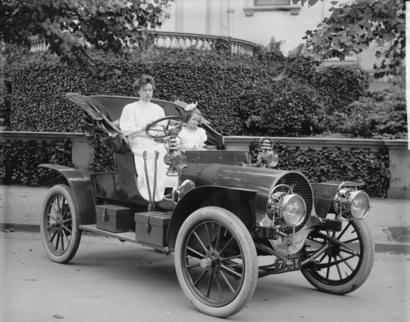
\includegraphics[width=\linewidth]{sample-franklin}
  \caption{1907 Franklin Model D roadster. Photograph by Harris \&
    Ewing, Inc. [Public domain], via Wikimedia
    Commons. (\url{https://goo.gl/VLCRBB}).}
  \Description{A woman and a girl in white dresses sit in an open car.}
\end{figure}

Your figures should contain a caption which describes the figure to
the reader.

CTANacmart}.
  Artifacts: \cite{R} and \cite{UMassCitations}.

\section{Acknowledgments}

Identification of funding sources and other support, and thanks to
individuals and groups that assisted in the research and the
preparation of the work should be included in an acknowledgment
section, which is placed just before the reference section in your
document.

This section has a special environment:
\begin{verbatim}
  \begin{acks}
  ...
  \end{acks}
\end{verbatim}
so that the information contained therein can be more easily collected
during the article metadata extraction phase, and to ensure
consistency in the spelling of the section heading.

Authors should not prepare this section as a numbered or unnumbered {\verb|\section|}; please use the ``{\verb|acks|}'' environment.

\section{Appendices}

If your work needs an appendix, add it before the
``\verb|\end{document}|'' command at the conclusion of your source
document.

Start the appendix with the ``\verb|appendix|'' command:
\begin{verbatim}
  \appendix
\end{verbatim}
and note that in the appendix, sections are lettered, not
numbered. This document has two appendices, demonstrating the section
and subsection identification method.

\section{Multi-language papers}

Papers may be written in languages other than English or include
titles, subtitles, keywords and abstracts in different languages (as a
rule, a paper in a language other than English should include an
English title and an English abstract).  Use \verb|language=...| for
every language used in the paper.  The last language indicated is the
main language of the paper.  For example, a French paper with
additional titles and abstracts in English and German may start with
the following command
\begin{verbatim}
\documentclass[sigconf, language=english, language=german,
               language=french]{acmart}
\end{verbatim}

The title, subtitle, keywords and abstract will be typeset in the main
language of the paper.  The commands \verb|\translatedXXX|, \verb|XXX|
begin title, subtitle and keywords, can be used to set these elements
in the other languages.  The environment \verb|translatedabstract| is
used to set the translation of the abstract.  These commands and
environment have a mandatory first argument: the language of the
second argument.  See \verb|sample-sigconf-i13n.tex| file for examples
of their usage.

\section{SIGCHI Extended Abstracts}

The ``\verb|sigchi-a|'' template style (available only in \LaTeX\ and
not in Word) produces a landscape-orientation formatted article, with
a wide left margin. Three environments are available for use with the
``\verb|sigchi-a|'' template style, and produce formatted output in
the margin:
\begin{description}
\item[\texttt{sidebar}:]  Place formatted text in the margin.
\item[\texttt{marginfigure}:] Place a figure in the margin.
\item[\texttt{margintable}:] Place a table in the margin.
\end{description}

%%
%% The acknowledgments section is defined using the "acks" environment
%% (and NOT an unnumbered section). This ensures the proper
%% identification of the section in the article metadata, and the
%% consistent spelling of the heading.
\begin{acks}
To Robert, for the bagels and explaining CMYK and color spaces.
\end{acks}

%%
%% The next two lines define the bibliography style to be used, and
%% the bibliography file.
\bibliographystyle{ACM-Reference-Format}
\bibliography{sample-base}


%%
%% If your work has an appendix, this is the place to put it.
\appendix

\section{Research Methods}

\subsection{Part One}

Lorem ipsum dolor sit amet, consectetur adipiscing elit. Morbi
malesuada, quam in pulvinar varius, metus nunc fermentum urna, id
sollicitudin purus odio sit amet enim. Aliquam ullamcorper eu ipsum
vel mollis. Curabitur quis dictum nisl. Phasellus vel semper risus, et
lacinia dolor. Integer ultricies commodo sem nec semper.

\subsection{Part Two}

Etiam commodo feugiat nisl pulvinar pellentesque. Etiam auctor sodales
ligula, non varius nibh pulvinar semper. Suspendisse nec lectus non
ipsum convallis congue hendrerit vitae sapien. Donec at laoreet
eros. Vivamus non purus placerat, scelerisque diam eu, cursus
ante. Etiam aliquam tortor auctor efficitur mattis.

\section{Online Resources}

Nam id fermentum dui. Suspendisse sagittis tortor a nulla mollis, in
pulvinar ex pretium. Sed interdum orci quis metus euismod, et sagittis
enim maximus. Vestibulum gravida massa ut felis suscipit
congue. Quisque mattis elit a risus ultrices commodo venenatis eget
dui. Etiam sagittis eleifend elementum.

Nam interdum magna at lectus dignissim, ac dignissim lorem
rhoncus. Maecenas eu arcu ac neque placerat aliquam. Nunc pulvinar
massa et mattis lacinia.

\end{document}
\endinput
%%
%% End of file `sample-sigconf.tex'.
